\documentclass[__main__.tex]{subfiles}

\newcommand{\stp}{\operatorname{stp}}
\newcommand{\Hom}{\operatorname{Hom}}
\begin{document}

\qtitle{43}
Схема метода конечных сумм для численного решения линейных уравнений в функциональных банаховых пространствах, критерий корректности этой схемы; пример численного решения методом конечных сумм интегрального уравнения Фредгольма 2-го рода с симметричным гладким аналитически заданным ядром.\\

Рассмотрим банаховы пространства $Y_0$ и $Z_0$ и $\hat{F}\colon{Y_0\rightarrow Z_0}$ -- линейный оператор, причем $D(\hat{F})=X_0$ и $E(\hat{F})=W_0$. Введем табуляции пространств $X_0$: $\hat\psi_{(\cdot)}=\left\{ \hat{\pi}_k\in\Hom(Y_0,{^>\mathbb{R}^{n_k}_{*}}) \right\}$ и $W_0$: $\hat{\Omega}_{(\cdot)}=\left\{ \hat\Omega_k\in\Hom(Z_0,{^>\mathbb{R}^{m_k}_{*}}) \right\}$. Для $\forall k\in\mathbb{N}$ определим матрицу $F_k\in L(\mathbb{R},n_k,m_k)$ размера $(n_k\times m_k)$ и соответствующий ей оператор $\hat{F}_k\in\Hom({^>\mathbb{R}^{m_k}},{^>\mathbb{R}^{n_k}})$.

\begin{definition}
Говорят, что $F_k$ -- табулирование оператора $\hat{F}$, если $\forall x\in X_0 \lim\limits_{n\rightarrow\infty}\Vert(\hat{F}_k\circ\hat\pi_{k}\circ\hat{F})(x)\Vert=0$
\end{definition}

\begin{figure}[h]
\centering
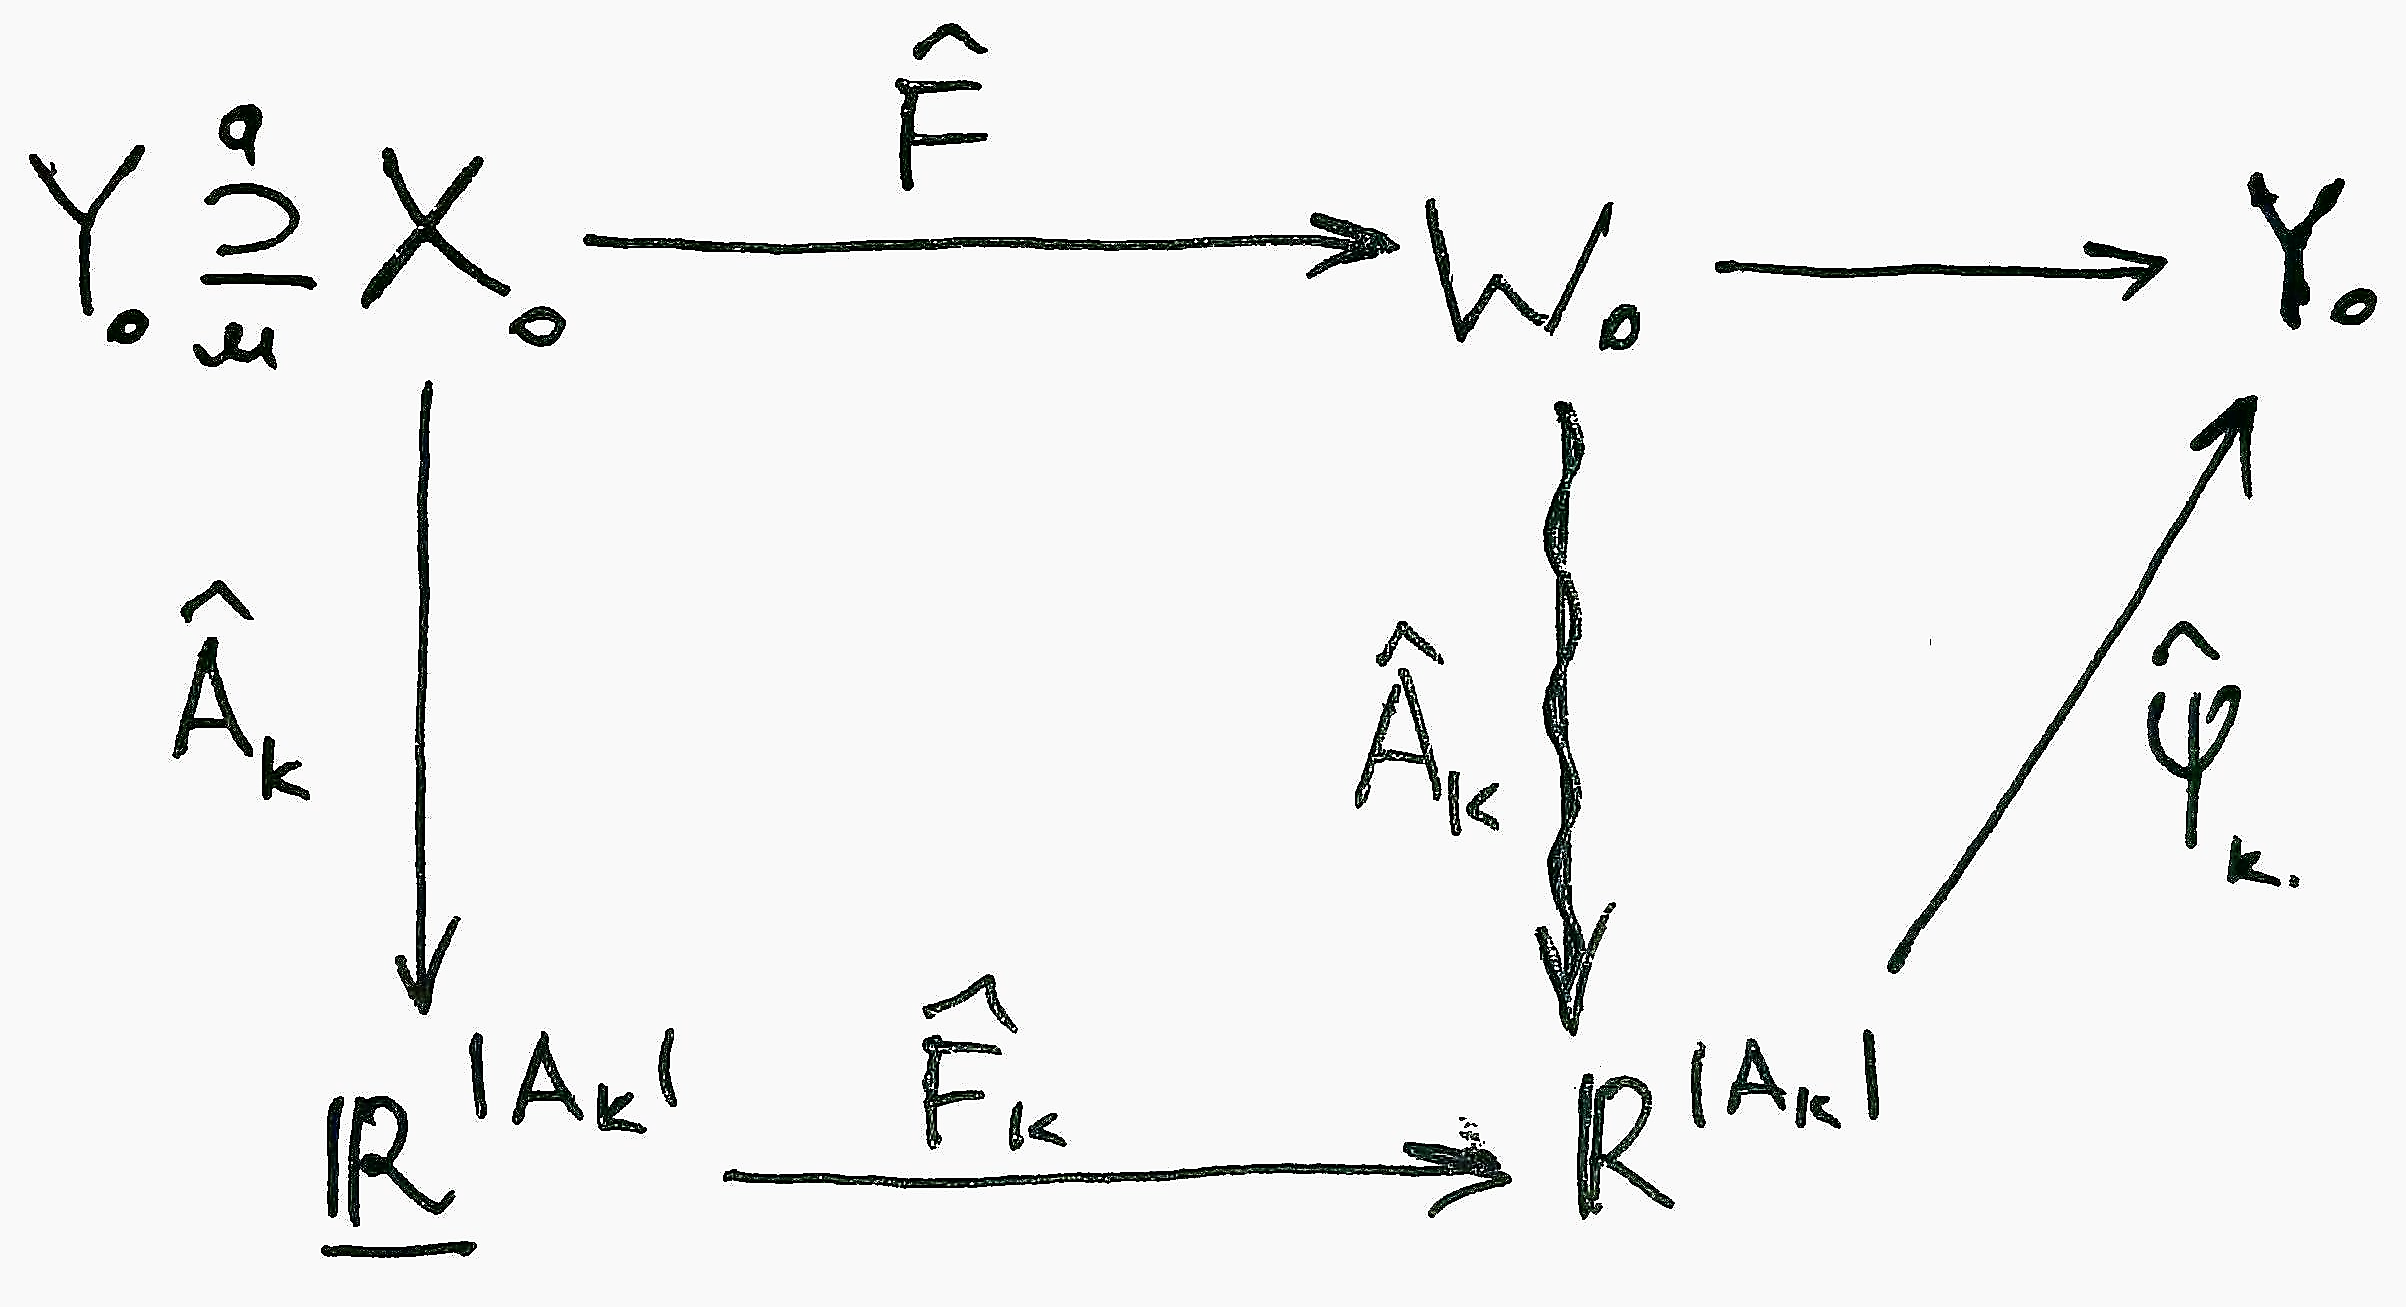
\includegraphics[width=.4\linewidth]{43-scheme.png}
\end{figure}

В случае функциональных банаховых пространств $X_0=C^{1}\left([a,b],\mathbb{R}\right)$ и $Z_0=C\left([a,b],\mathbb{R}\right)$ рассмотрим линейный интегральный оператор $\hat{F}$ с гладким ядром $K(x,t)$: $\hat{F}(x)=\int\limits_{a}^{b}K(x,t)x(t)dt$, тогда, задав устойчивую равномерную сетку $A_k$, можем перейти к конечной сумме:
\begin{gather}
\forall{i\in\overline{1,k}}\colon
\left.\hat{F}(x)\right|_{x_i}
\approx
\sum_{j=1}^{k}K(x_i,t_j)x(t_j)\stp(A_k),
\end{gather}
где матрица $\hat{F}_k$ примет вид:
\begin{gather}
F_k = \left( K(x_i,t_j)\stp(A_k) \right)_{k\times k}
\end{gather}

Рассмотрим уравнение Фредгольма 2-го рода с симметричным гладким аналитически заданным ядром $K(x,t)$:
\begin{gather}
\hat{F}(\varphi)=\varphi(x)-\lambda\int\limits_{a}^{b}K(x,t)\varphi(t)dt=f(x),
\end{gather}
Рассмотрим двумерную центрально-равномерную сетку $A \times B = \left<(x_i,t_j)|x_i\in A\wedge t_j\in B\right>$, с шагом $\stp(A)=\stp(B)=h$, тогда интегральное уравнение можно заменить СЛАУ при помощи квадратурной формулы прямоугольников:
\begin{flalign}
\begin{split}
&
\varphi(x_i)-\lambda\sum_{j=1}^{n}K(x_i,t_j)\varphi(t_j)h = f(x_i)
\Longrightarrow\\
\Longrightarrow
&\left(\delta_{ij}-\lambda h K_{ij}\right)\varphi^j=f_i
\Longrightarrow
M_{ij}\varphi^{j}=f_i
\end{split}
\end{flalign}
Решив СЛАУ, получим сеточную функцию ${^>\varphi}=\left[\varphi^1,\dots,\varphi^n\right>$, индуцирующую при помощи интерполяции приближенное решение исходного уравнения.

\end{document}